\documentclass[12pt,twoside,a4paper]{article}


\usepackage[usenames,dvipsnames]{color}
\usepackage{graphics}
\usepackage{textcomp}
\usepackage[official]{eurosym}
\usepackage{amsmath}
\usepackage{amssymb}
\usepackage{amsthm}
\usepackage[pdftex]{graphicx}
\usepackage{sidecap}
%\usepackage{subfigure} - this is obsolete


\usepackage{verbatim}
%\usepackage[small]{caption}
\usepackage[font={small,it}]{caption}
\usepackage[font={small,it},labelformat=simple]{subcaption}
\renewcommand\thesubfigure{(\alph{subfigure})}
%\usepackage{subcaption}
\usepackage{rotating}
\usepackage{listings}
\usepackage{fancyvrb}
\VerbatimFootnotes
\usepackage[toc,page]{appendix}
\usepackage{lscape}
\usepackage{placeins}
\usepackage[all]{xy}
\usepackage{wrapfig}
\usepackage{multicol}
\usepackage{multirow}
\usepackage{enumerate}
\usepackage{enumitem}
\usepackage{setspace}
\usepackage{nomencl}
\usepackage[stable]{footmisc}

\usepackage[linesnumbered,ruled,vlined]{algorithm2e}
\usepackage{algpseudocode} % To use algorithmicx




\usepackage{etex}
\usepackage{tkz-euclide}
\usepackage{tikz}
\usetikzlibrary{arrows}
\usetikzlibrary{decorations.markings}
\tikzset{->-/.style={decoration={
  markings,
  mark=at position #1 with {\arrow{>}}},postaction={decorate}}}

%\tikzset{->-/.style={decoration={
%  markings,
%  mark=at position 0.25 and 0.9 step 0.25 with {\arrow{>}}},postaction={decorate}}}

%\tikzset{->>>>-/.style={decoration={
%  markings,
%  mark=at position 0.25 with {\arrow{>}}},postaction={decorate}},
%  mark=at position 0.5 with {\arrow{>}}},postaction={decorate}};}

\usepackage[utf8]{inputenc}

% Used to create tree diagrams
\usepackage{forest}

% Silence warnings by hyper link stuff.
\usepackage{silence}
\WarningFilter{hyperref}{You have enabled option `breaklinks'.}

\PassOptionsToPackage{hyphens}{url}\usepackage[breaklinks]{hyperref}
%\usepackage[breaklinks]{hyperref}
\usepackage[hyphenbreaks]{breakurl}

\usepackage[sort&compress, % on multiple refs sort them and write as range
            capitalise, % Use Section not section etc.
            noabbrev, % Use Table not Tab. etc.
            nameinlink % Make the name (eg Section) part of the hyperlink
            ]{cleveref}

\usepackage{mathtools}

\usepackage[framemethod=TikZ]{mdframed} % For my framed boxes

% Call subsections sections
\crefname{subsection}{Section}{Sections}
\Crefname{subsection}{Section}{Sections}

% just use (...) for equations
\crefformat{equation}{#2(#1)#3}
\crefrangeformat{equation}{#3(#1)#4--#5(#2)#6}
\crefmultiformat{equation}{(#2#1#3)}{ and~(#2#1#3)}{, (#2#1#3)}{ and~(#2#1#3)}

% Except for start of sentences where we need to say "Equations"
\Crefformat{equation}{Equation~#2(#1)#3}
\Crefrangeformat{equation}{Equations~#3(#1)#4--#5(#2)#6}
\Crefmultiformat{equation}{Equations~(#2#1#3)}{ and~(#2#1#3)}{, (#2#1#3)}{ and~(#2#1#3)}


% a reference for "this X"
%\newcommand{\thisref}[1]{this \lcnamecref{#1}}
%\newcommand{\Thisref}[1]{This \lcnamecref{#1}}


%\usepackage[breaklinks=true]{hyperref}
%\PassOptionsToPackage{hyphens}{url}\usepackage{hyperref}

%\usepackage{hyperref}

\numberwithin{equation}{section}

% Used for figure environment, can now use [H] to put the
% figure right here and force text to go below it.
\usepackage{float}
\setcounter{secnumdepth}{3}
\setcounter{tocdepth}{3}

% biblatex setup
\usepackage[backend=biber,
  citestyle=numeric,
  firstinits=true, % Only print initials of first names
  isbn=false,
  doi=false,
  url=true, % for websites, see below for removing it from papers etc.
  backref=true, % print out the page number of reference
]{biblatex}

% clear urls for papers, proceedings, books
\AtEveryBibitem{%
  \ifentrytype{article}{%
    \clearfield{url}%
    \clearfield{urldate}%
    \clearfield{month}%
  }
  {}% no "else" operation
  %
  \ifentrytype{inproceedings}{%
    \clearfield{url}%
    \clearfield{urldate}%
    \clearfield{month}%
  }
  {}% no "else" operation
  % 
  \ifentrytype{book}{%
    \clearfield{url}%
    \clearfield{urldate}%
    \clearfield{month}%
  }
  {}% no "else" operation
  \ifentrytype{phdthesis}{%
    \clearfield{url}%
    \clearfield{urldate}%
    \clearfield{month}%
  }
  {}% no "else" operation


}


\renewbibmacro{in:}{%
  \ifentrytype{article}{}{\printtext{\bibstring{in}\intitlepunct}}}

% makes volume of journal bold and adds colon
\DeclareFieldFormat[article]{volume}{\textbf{#1}\addcolon\space}
% removes pagination (p./pp.) before page numbers
\DeclareFieldFormat{pages}{#1}

\DefineBibliographyStrings{english}{%
    backrefpage  = {see p.}, % for single page number
    backrefpages = {see pp.} % for multiple page numbers
}


% Add bibtex files
\addbibresource{library.bib}

% Change this for autoref
%\renewcommand{\chapterautorefname}{Chapter}
%\renewcommand{\figurename}{Figure}
%\renewcommand{\tablename}{Table}
%\renewcommand{\partname}{Part}
%\renewcommand{\appendixname}{Appendix}
%\equationname	
%Equation
%\Itemname	
%item
%\chaptername	
%chapter
%\sectionname	
%section
%\subsectionname	
%subsection
%\subsubsectionname	
%subsubsection
%\paragraphname	
%paragraph
%\Hfootnotename	
%footnote
%\AMSname	
%Equation
%\theoremname	
%Theorem
%\page	
%page
\makenomenclature
\DeclareMathOperator*{\Ext}{Ext. }

% Below are the spacing options.
%\doublespacing
%\singlespacing
%\onehalfspacing
%\setstretch{1.8}

\newtheorem{definition}{Definition}[section]
\newtheorem{proposition}{Proposition}[section]
\newtheorem{example}{Example}[section]
\newtheorem{theorem}{Theorem}[section]
\newtheorem{remark}{Remark}[section]
\newcommand{\pde}{partial differential equation}
\newcommand{\Pde}{Partial differential equation}
\newcommand{\pdes}{partial differential equations}
\newcommand{\Pdes}{Partial differential equations}
%\newcommand{\ul}[1]{\underline{#1}}
\newcommand{\degree}{^{\circ}}



%%%%%%%%%%%%%%%%%%%%%%%%%%%%%%%%%%%%%%%%%%%%%%%%%%%%%%%%%%%%%%%%%%%%%%%%%%%%
%%%%%%%%%%%%%%%%%%%%%%%%%%%%%%%%%%%%%%%%%%%%%%%%%%%%%%%%%%%%%%%%%%%%%%%%%%%%
%%%%%%%%%%%%%%%%%%%%%%%%%%%%%%%%%%%%%%%%%%%%%%%%%%%%%%%%%%%%%%%%%%%%%%%%%%%%
%%%%%%%%%% Words
\newcommand{\oomphlib}{\texttt{oomph-lib}}
\newcommand{\Oomphlib}{\texttt{Oomph-lib}}
\newcommand{\SuperLU}{\texttt{SuperLU}}
\newcommand{\faceelement}{\texttt{FaceElement}}
\newcommand{\infsup}{\emph{inf-sup}}

%%%%%%%%%%%%%%%%%%%%%%%%%%%%%%%%%%%%%%%%%%%%%%%%%%%%%%%%%%%%%%%%%%%%%%%%%%%%
%%%%%%%%%%%%%%%%%%%%%%%%%%%%%%%%%%%%%%%%%%%%%%%%%%%%%%%%%%%%%%%%%%%%%%%%%%%%
%%%%%%%%%%%%%%%%%%%%%%%%%%%%%%%%%%%%%%%%%%%%%%%%%%%%%%%%%%%%%%%%%%%%%%%%%%%%
%% Maths stuff, these should always go in math mode.

% Generic
\newcommand{\realnumbers}{\mathbb{R}} % Real numbers
\newcommand{\complexnumbers}{\mathbb{C}} % Real numbers
\newcommand{\realvectors}[1]{\mathbb{R}^{#1}} % Real numbers
\newcommand{\realmatrices}[2]{\mathbb{R}^{#1 \times #2}} % Real numbers
\newcommand{\tolgeneral}{\varepsilon} % General tol for iterative methods
\newcommand{\tolnewton}{\varepsilon_N} % Newton tolerance
\newcommand{\tolkrylov}{\varepsilon_K} % Krylov/GMRES tolerance
\newcommand{\toltime}{\varepsilon_T} % adaptivetime tolerance
\newcommand{\tolnumnewton}{10^{-6}}
\newcommand{\tolnumkrylov}{10^{-6}}
\newcommand{\tolnumtime}{10^{-4}}
\newcommand{\bigo}[1]{\mathcal{O}(#1)} % Big-O notation
\newcommand{\pow}[1]{^{#1}}
\newcommand{\inv}{\pow{-1}}
\newcommand{\tran}{^{T}}



% Stuff about domains%%%%%%%%%%%%%%%%%%%%%%%%%%%%%%%%%%%%%%%%%%%%%%%%%%%%%%%
\newcommand{\domain}{\Omega}

\newcommand{\angleofrot}{\alpha}
\newcommand{\rotdomain}{\Omega^{[\angleofrot]}}
\newcommand{\rotdomainang}[1]{\Omega^{[#1]}}

% Boundaries
\newcommand{\bound}{\partial\domain} % Generic boundary
\newcommand{\genconstrainedbound}{\bound_\lambda} % Constrained boundary
\newcommand{\charbound}{\bound_{c}} % Characteristic boundary
\newcommand{\inbound}{\bound_{i}} % Inflow
\newcommand{\outbound}{\bound_{o}} % Outflow
\newcommand{\tractvec}{T}



% Finite element discretisation stuff
\newcommand{\eleq}[1]{\mathbf{Q}_{#1}}
\newcommand{\elep}[1]{\mathbf{P}_{#1}}
\newcommand{\taylorhood}{\eleq{2}-\eleq{1}}
\newcommand{\ijdim}{\text{for } i,j = 1,2\,[,3]}
\newcommand{\idim}{\text{for } i = 1,2\,[,3]}
\newcommand{\jdim}{\text{for } j = 1,2\,[,3]}
\newcommand{\vsol}{\psi}
\newcommand{\psol}{\varphi}
\newcommand{\vtest}{\Phi}
\newcommand{\ptest}{\chi}
\newcommand{\dirichleti}{\Omega_{D_i}}
\newcommand{\neumanni}{\Omega_{N_i}}
\newcommand{\pfrac}[2]{\frac{\partial #1}{\partial #2}}


% Absolute value and norms
\DeclarePairedDelimiter\abs{\lvert}{\rvert}%
\DeclarePairedDelimiter\norm{\lVert}{\rVert}%
% Swap the definition of \abs* and \norm*, so that \abs
% and \norm resizes the size of the brackets, and the 
% starred version does not.
\makeatletter
\let\oldabs\abs
\def\abs{\@ifstar{\oldabs}{\oldabs*}}
%
\let\oldnorm\norm
\def\norm{\@ifstar{\oldnorm}{\oldnorm*}}
\makeatother

% Systems of linear equations
\newcommand{\approxchi}{\chi}
\newcommand{\approxx}[1]{\bar{\approxchi}^{(#1)}} % For the approximate solution
\newcommand{\comapproxx}[1]{\approxchi^{(#1)}}
\newcommand{\exactx}{\bar{x}^*}
% Ax = b %%%%%%%%%%%%%%%%%%%%%%%%%%%%
\newcommand{\linA}{A} % Matrix A
\newcommand{\linB}{B} % Matrix A
\newcommand{\linC}{C} % Matrix A
\newcommand{\linD}{D} % Matrix A
\newcommand{\linE}{E} % Matrix A
\newcommand{\linF}{F} % Matrix A
\newcommand{\linG}{G} % Matrix A
\newcommand{\linH}{H} % Matrix A
\newcommand{\linI}{I} % Matrix A
\newcommand{\linJ}{J} % Matrix A
\newcommand{\linK}{K} % Matrix A
\newcommand{\linL}{L} % Matrix A
\newcommand{\linM}{M} % Matrix A
\newcommand{\linN}{N} % Matrix A
\newcommand{\linO}{O} % Matrix A
\newcommand{\linP}{P} % Matrix A
\newcommand{\linQ}{Q} % Matrix A
\newcommand{\linR}{R} % Matrix A
\newcommand{\linS}{S} % Matrix A
\newcommand{\linT}{T} % Matrix A
\newcommand{\linU}{U} % Matrix A
\newcommand{\linV}{V} % Matrix A
\newcommand{\linW}{W} % Matrix A
\newcommand{\linX}{X} % Matrix A
\newcommand{\linY}{Y} % Matrix A
\newcommand{\linZ}{Z} % Matrix A


\newcommand{\itermat}{\linG{}}
\newcommand{\itermatwj}{\linG{}_{J_{\omega}}}
\newcommand{\eye}{\linI{}}

\newcommand{\bxx}{11}
\newcommand{\bxxc}{1\hat{1}}
\newcommand{\bxy}{12}
\newcommand{\bxyc}{1\hat{2}}

\newcommand{\bxcx}{\hat{1}1}
\newcommand{\bxcxc}{\hat{1}\hat{1}}
\newcommand{\bxcy}{\hat{1}2}
\newcommand{\bxcyc}{\hat{1}\hat{2}}

\newcommand{\byx}{21}
\newcommand{\byxc}{2\hat{1}}
\newcommand{\byy}{22}
\newcommand{\byyc}{2\hat{2}}

\newcommand{\bycx}{\hat{2}1}
\newcommand{\bycxc}{\hat{2}\hat{1}}
\newcommand{\bycy}{\hat{2}2}
\newcommand{\bycyc}{\hat{2}\hat{2}}

\newcommand{\bx}{1}
\newcommand{\by}{2}
\newcommand{\bxc}{\hat{1}}
\newcommand{\byc}{\hat{2}}

%\newcommand{\xcx}{\hat{1}1}
%\newcommand{\xcxc}{\hat{1}\hat{1}}
%\newcommand{\yy}{11}
%\newcommand{\ycy}{\hat{1}1}
%\newcommand{\yyc}{1\hat{1}}
%\newcommand{\ycyc}{\hat{1}\hat{1}}



% vectors in linear algebra has a bar on top.
\newcommand{\linvec}[1]{\bar{#1}}
\newcommand{\lina}{\linvec{a}} % vector a
\newcommand{\linb}{\linvec{b}} % vector b
\newcommand{\linc}{\linvec{c}} % c
\newcommand{\lind}{\linvec{d}} % d
\newcommand{\linee}{\linvec{e}} % d
\newcommand{\linf}{\linvec{f}} % d
\newcommand{\ling}{\linvec{g}} % d
\newcommand{\linh}{\linvec{h}} % d
\newcommand{\lini}{\linvec{i}} % d
\newcommand{\linj}{\linvec{j}} % d
\newcommand{\link}{\linvec{k}} % d
\newcommand{\linl}{\linvec{l}} % \line is defined already
\newcommand{\linm}{\linvec{m}} % d
\newcommand{\linn}{\linvec{n}} % d
\newcommand{\lino}{\linvec{o}} % d
\newcommand{\linp}{\linvec{p}} % d
\newcommand{\linx}{\linvec{x}} % 
\newcommand{\liny}{\linvec{y}} % 
\newcommand{\linz}{\linvec{z}} % 
\newcommand{\linr}{\linvec{r}} % r - normally used for residuals
\newcommand{\linu}{\linvec{u}} % r - normally used for residuals
\newcommand{\linv}{\linvec{v}} % r - normally used for residuals
\newcommand{\linw}{\linvec{w}} % r - normally used for residuals

\newcommand{\tangvec}{\hat{t}^{\,i}}
\newcommand{\normvec}{\hat{n}}
\newcommand{\constrainedvec}{\hat{c}}


\newcommand{\kspace}[1]{\mathcal{K}_#1}
\newcommand{\knspace}{\kspace{n}}
\newcommand{\fwj}{\linf{}_{J_{\omega}}}
\newcommand{\numitererror}[1]{\lind{}^{(#1)}}
\newcommand{\kthitererror}{\numitererror{k}}
\newcommand{\initialitererror}{\numitererror{0}}

\newcommand{\tenpower}[1]{\times10^{#1}}



\newcommand{\coma}{a} % vector a
\newcommand{\comb}{b} % vector b
\newcommand{\comc}{c} % c
\newcommand{\comd}{d} % d
\newcommand{\comee}{e} % \line is defined already
\newcommand{\comf}{f} % d
\newcommand{\comg}{g} % d
\newcommand{\comh}{h} % d
\newcommand{\comi}{i} % d
\newcommand{\comj}{j} % d
\newcommand{\comk}{k} % d
\newcommand{\coml}{l} % d
\newcommand{\comm}{m} % d
\newcommand{\comn}{n} % d
\newcommand{\como}{o} % d
\newcommand{\comp}{p} % d
\newcommand{\comx}{x} % 
\newcommand{\comy}{y} % 
\newcommand{\comz}{z} % 
\newcommand{\comr}{r} % r - normally used for residuals
\newcommand{\comu}{u} % r - normally used for residuals
\newcommand{\comv}{v} % r - normally used for residuals
\newcommand{\comw}{w} % r - normally used for residuals

\newcommand{\pobound}{\partial\Omega_P}
\newcommand{\tfbound}{\partial\Omega_T}
\newcommand{\constrainedbound}{\partial\Omega_\lambda}


\newcommand{\linAx}{\linA{}\linx{}}  %Ax = b
\newcommand{\linAexactx}{\linA{}\exactx{}} %A \tild{x}^*
\newcommand{\linAappoxx}[1]{\linA{}\approxx{#1}}%A \tilde{x}^#1

% This is quite specific to my thesis, this is the dimensions of my
% generic linear system Ax = b
% Dimensions of A is n x n, x is n, b is n
\newcommand{\genrowdim}{n}
\newcommand{\gencoldim}{m}
\newcommand{\dimlinA}{\realmatrices{n}{n}}
\newcommand{\dimlinx}{\realvectors{n}}
\newcommand{\forioneton}{i = 1,\ldots,\genrowdim{}}
\newcommand{\numlgrdof}{N_{\Lambda}} 
\newcommand{\numpdof}{N_p}
\newcommand{\numnsdof}{N_{ns}}
\newcommand{\numvdof}{N_{u}}
\newcommand{\wscaling}{\sigma}
% Function spaces
\newcommand{\Lpspace}[1]{L^{#1}}
\newcommand{\Ltwo}{\Lpspace{2}}
\newcommand{\genjac}{\mathcal{F}}
\newcommand{\nsjac}{\mathcal{F}_{ns}}
\newcommand{\modnsjac}{\widehat{\mathcal{F}}_{ns}}
\newcommand{\genprec}{\mathcal{P}}
\newcommand{\precE}{\mathcal{P}_E}
\newcommand{\precLSC}{\mathcal{P}_{LSC}}
\newcommand{\preciLSC}{\widehat{\mathcal{P}}_{LSC}}
\newcommand{\subL}{\widehat{L}}
\newcommand{\gendiagM}{\widehat{D}_M}
\newcommand{\diagvmm}{\hat{M}}
\newcommand{\modF}{\widehat{F}}

\newcommand{\reyparam}{Re}
\newcommand{\subprobeig}{\tilde{\lambda}}
\newcommand{\seigi}{\tilde{\lambda}_i}
\newcommand{\seigr}{\tilde{\lambda}_r}

%\renewcommand\thesubfigure{(\alph{subfigure})}

%\makeatletter
%\let\latex@xfloat=\@xfloat
%\def\@xfloat #1[#2]{%
%  \latex@xfloat #1[#2]%
%  \def\baselinestretch{1}
%  \@normalsize\normalsize
%  \normalsize
%}
%\makeatother

% This is the standardone inch all around border.
%\usepackage{fullpage}

% This is what I've made myself - max space used, for Tisseur cw.
% For most stand alone work, use this one.
%\setlength{\abovecaptionskip}{5pt}
%\setlength{\belowcaptionskip}{20pt}
%\setlength{\topmargin}{-1in}
%\setlength{\textheight}{9.75in}
%\setlength{\oddsidemargin}{-0.25in}
%\setlength{\textwidth}{7in}

% This is the geometry package... apparently good!
%\usepackage[left=2cm,top=4cm,right=2cm]{geometry}
%\usepackage[a4paper]{geometry}
%\geometry{top=1.0in, bottom=1.0in, left=1.6in, right=1.0in}

%\setlength{\abovecaptionskip}{-1pt} % required for picture captions

\definecolor{mygreen}{rgb}{0,0.6,0}
\definecolor{mygray}{rgb}{0.5,0.5,0.5}
\definecolor{mymauve}{rgb}{0.58,0,0.82}
\definecolor{listinggray}{gray}{0.9}
\definecolor{lstbcolor}{rgb}{0.94,0.94,0.94}



% Common listing stuff
\lstset{
  breaklines=true, % Auto wrap lines
  postbreak=\raisebox{0ex}[0ex][0ex]{\ensuremath{\color{red}\hookrightarrow\space}},%for placing a red arrow at the beginning of the broken line to emphasize the line break. 
  escapeinside={(*@}{@*)},
  backgroundcolor=\color{lstbcolor},
  captionpos=b, % sets the caption-position to bottom
  extendedchars=true, % lets you use non-ASCII characters; 
                      % for 8-bits encodings only, 
                      % does not work with UTF-8
  numbers=left, % where to put the line-numbers; 
                % possible values are (none, left, right)
  numbersep=6pt, % how far the line-numbers are from the code
  numberstyle=\color{mygray}, % the style that is used for the 
                                   % line-numbers
  stepnumber=2, 
  frame=single,
  basicstyle=\footnotesize\ttfamily,
  commentstyle=\itshape\color{blue!80!white},
  keywordstyle=\bfseries\color{orange!90!black},
  stringstyle=\color{orange},
  belowcaptionskip=1\baselineskip,
  showstringspaces=false,
  tabsize=2 % sets default tabsize to 2 spaces
}


\lstdefinestyle{raycodecpp}{
  rangebeginprefix=///\ Start\ of\ ,
  rangeendprefix=///\ End\ of\ ,
  includerangemarker=true,
  identifierstyle=,%\color{blue},
  language=C++
%  title=\lstname % show the filename of files included with 
%                 %\lstinputlisting; also try caption instead of title
}


\lstdefinestyle{raycodebash}{
  rangebeginprefix=\#\#\#\ Start\ of\ ,
  rangeendprefix=\#\#\#\ End\ of\ ,
  includerangemarker=true,
  identifierstyle=,%\color{blue},
  language=bash
%  title=\lstname % show the filename of files included with 
%                 %\lstinputlisting; also try caption instead of title
}

\lstdefinestyle{raycodetetgenpoly}{
  rangebeginprefix=\#\#\#\ Start\ of\ ,
  rangeendprefix=\#\#\#\ End\ of\ ,
  includerangemarker=true,
  identifierstyle=,%\color{blue},
  morecomment=[l]{\#}
}




% Doing boarder matrices
\makeatletter
\def\bbordermatrix#1{\begingroup \m@th
  \@tempdima 4.75\p@
  \setbox\z@\vbox{%
    \def\cr{\crcr\noalign{\kern2\p@\global\let\cr\endline}}%
    \ialign{$##$\hfil\kern2\p@\kern\@tempdima&\thinspace\hfil$##$\hfil
      &&\quad\hfil$##$\hfil\crcr
      \omit\strut\hfil\crcr\noalign{\kern-\baselineskip}%
      #1\crcr\omit\strut\cr}}%
  \setbox\tw@\vbox{\unvcopy\z@\global\setbox\@ne\lastbox}%
  \setbox\tw@\hbox{\unhbox\@ne\unskip\global\setbox\@ne\lastbox}%
  \setbox\tw@\hbox{$\kern\wd\@ne\kern-\@tempdima\left[\kern-\wd\@ne
    \global\setbox\@ne\vbox{\box\@ne\kern2\p@}%
    \vcenter{\kern-\ht\@ne\unvbox\z@\kern-\baselineskip}\,\right]$}%
  \null\;\vbox{\kern\ht\@ne\box\tw@}\endgroup}
\makeatother

%\renewcommand*{\algorithmcfname}{ASM Spec.}% Algorithm name
%\usepackage{dcounter}% http://ctan.org/pkg/dcounter
%\counterstyle{<section>}%
%\DeclareDynamicCounter{algocf}% <- algocf will be 'dynamic' within <section>

\newcounter{preccounter}
\newenvironment{preconditioner}[1][h]
  {\refstepcounter{preccounter}
    \renewcommand*{\algorithmcfname}{Preconditioner}
  \LinesNotNumbered
    \LinesNumberedHidden
    \begin{algorithm}[#1]
  \DontPrintSemicolon 
      \renewcommand\thealgocf{\arabic{preccounter}}}
  {\end{algorithm}\addtocounter{algocf}{-1}}
\newcommand{\precref}[1]{Preconditioner \ref{#1}}


\newcommand*{\threesim}{
\mathrel{\vcenter{\offinterlineskip
\hbox{$\sim$}\vskip-.35ex\hbox{$\sim$}\vskip-.35ex\hbox{$\sim$}}}}


%\newcounter{preccounter}
%\newenvironment{Preconditioner}
%  {\refstepcounter{preccounter}%
%    \renewcommand*{\algorithmcfname}{Preconditioner}%
%    \begin{algorithm}\renewcommand\thealgocf{\arabic{preccounter}}}
%  {\end{algorithm}\addtocounter{algocf}{-1}}

%\newcommand{\precref}[1]{Preconditioner \ref{#1}}
%\newcounter{preccount}
%\newcounter{temp}
%
%\newenvironment{preccount}[1][ps]{%
%  \setcounter{temp}{\value{algorithm}}%
%  \setcounter{algorithm}{\value{preccount}}%
%  \refstepcounter{preccount}%
%  \begin{algorithm}[#1]%
%    \floatname{algorithm}{Preconditioner}%
%  }{\end{algorithm}\setcounter{algorithm}{\value{temp}}}
%
%\floatname{preccount}{Preconditioner}
%\crefname{hdps}{preconditioner}{preconditioners}
%\Crefname{hdps}{{Preconditioner}{Preconditioners}

%\crefname{algocf}{alg.}{algs.}
%\Crefname{algocf}{Algo}{Algos}
%\crefalias{hdps}{algocf}



% new environment syntax:
%\newenvironment{name}[num]{before}{after}
%\newcounter{precc}
%\newenvironment{preconditioner}
%  {\stepcounter{precc}
%    \renewcommand{\algorithmcfname}{Preconditioner}
%    \begin{algorithm}\renewcommand\thealgocf{\arabic{precc}}}
%  {\end{algorithm}\addtocounter{algocf}{-1}}
%% Set up the clever ref counter.
%\crefname{algocf}{Preconditioner}{preconditioners}
%\Crefname{algocf}{Preconditioner}{preconditioners}
%\renewcommand*{\algorithmcfname}{}% Algorithm name
%\usepackage{dcounter}% http://ctan.org/pkg/dcounter
%\counterstyle{<section>}%
%\DeclareDynamicCounter{algocf}% <- algocf will be 'dynamic' within <section>




\immediate\write18{./testshell.sh > testshell.tex}




%%%%%%%%%%%%%%%%%%%%%%%%%%%%%%%%%%%%%%%%%%%%%%%%%%%%%%%%%%%%%%%%%%%%%%%%%%%%
%%%%%%%%%%%%%%%%%%%%%%%%%%%%%%%%%%%%%%%%%%%%%%%%%%%%%%%%%%%%%%%%%%%%%%%%%%%%
%%%%%%%%%%%%%%%%%%%%%%%%%%%%%%%%%%%%%%%%%%%%%%%%%%%%%%%%%%%%%%%%%%%%%%%%%%%%

\newcommand{\tetp}{\texttt{-p}}
\newcommand{\tetq}{\texttt{-q}}
\newcommand{\tetr}{\texttt{-r}}
\newcommand{\teta}{\texttt{-a}}
\newcommand{\tetm}{\texttt{-m}}
\newcommand{\tetg}{\texttt{-g}}
\newcommand{\tetk}{\texttt{-k}}
\newcommand{\teti}{\texttt{-i}}
\newcommand{\tetw}{\texttt{-w}}
\newcommand{\tetA}{\texttt{-A}}
\newcommand{\tetB}{\texttt{-B}}
\newcommand{\tetR}{\texttt{-R}}
\newcommand{\tetV}{\texttt{-V}}
\newcommand{\tetI}{\texttt{-I}}

\begin{document}

%% Title stuff
\title{A note on TetGen with \oomphlib{} \\Using a unit cube example.}
\author{Raymon White}
\maketitle
%% End of title stuff

%\begin{abstract}
%This article attempts summarise the use of tetgen with \oomphlib{}.
%We base out example on a unit cube....
%\end{abstract}
TetGen is a quality tetrahedral mesh generator and a 3D Delaunay
triangulator. It is able to generate tetrahedral meshes of any 3D polyhedral
domains, including exact constrained Delaunay tetrahedralisations, boundary
conforming Delaunay meshes, and Voronoi partitions. Various features to
generate good quality and adaptive tetrahedral meshes suitable for numerical
methods, such as finite element or finite volume methods are provided.

\oomphlib{} is an object-oriented, open-source finite-element library for
the simulation of multi- (and single-)physics problems. An interface for
TetGen is implement.

This article attempts summarise the use of TetGen with \oomphlib{}.
We base our example on a unit cube and only cover features we require.
For a complete overview of the capabilities of Tetgen, see~\cite{Si2013}.

\section[TetGen input file (.poly file)]
{TetGen input file (.poly file)~\cite[p. 55]{Si2013}}
We want to create a unit cube as per \cref{fig:unitcube}.
% Annular wedge diagram %%%%%%%%%%%%%%%%%%%%%%%%%%%%%%%%%%%%%%%%%%%%%%%%%%%%
\begin{figure}[H] % !htbp
  \centering
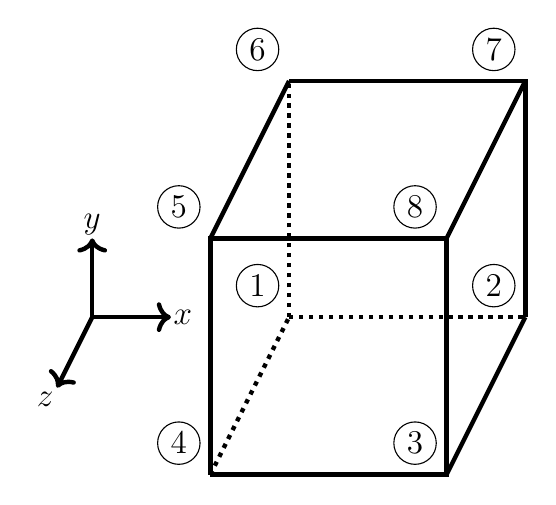
\begin{tikzpicture}
%  \draw[help lines] (0,0) grid (10,10);

\begin{scope}

%% Draw the cube first, axes later
\pgfmathsetmacro\FRONTBOTTOMLEFTX{0.0}
\pgfmathsetmacro\FRONTBOTTOMLEFTY{0.0}
\pgfmathsetmacro\CUBESIZE{3}

\pgfmathsetmacro\fbotleftX{\FRONTBOTTOMLEFTX}
\pgfmathsetmacro\fbotleftY{\FRONTBOTTOMLEFTY}
\pgfmathsetmacro\fbotrightX{\FRONTBOTTOMLEFTX+\CUBESIZE}
\pgfmathsetmacro\fbotrightY{\FRONTBOTTOMLEFTY}
\pgfmathsetmacro\ftopleftX{\FRONTBOTTOMLEFTX}
\pgfmathsetmacro\ftopleftY{\FRONTBOTTOMLEFTY+\CUBESIZE}
\pgfmathsetmacro\ftoprightX{\FRONTBOTTOMLEFTX+\CUBESIZE}
\pgfmathsetmacro\ftoprightY{\FRONTBOTTOMLEFTY+\CUBESIZE}

\coordinate (fbotleft) at (\fbotleftX,\fbotleftY);
\coordinate (fbotright) at (\fbotrightX,\fbotrightY);
\coordinate (ftopleft) at (\ftopleftX,\ftopleftY);
\coordinate (ftopright) at (\ftoprightX,\ftoprightY);

\draw[ultra thick] 
(fbotleft)--(fbotright)--(ftopright)--(ftopleft)--(fbotleft);

% How much is the back shifted from the front by?
\pgfmathsetmacro\FBSHIFTX{1}
\pgfmathsetmacro\FBSHIFTY{2}
\pgfmathsetmacro\BACKBOTTOMLEFTX{\FRONTBOTTOMLEFTX+\FBSHIFTX}
\pgfmathsetmacro\BACKBOTTOMLEFTY{\FRONTBOTTOMLEFTY+\FBSHIFTY}

\pgfmathsetmacro\bbotleftX{\BACKBOTTOMLEFTX}
\pgfmathsetmacro\bbotleftY{\BACKBOTTOMLEFTY}
\pgfmathsetmacro\bbotrightX{\BACKBOTTOMLEFTX+\CUBESIZE}
\pgfmathsetmacro\bbotrightY{\BACKBOTTOMLEFTY}
\pgfmathsetmacro\btopleftX{\BACKBOTTOMLEFTX}
\pgfmathsetmacro\btopleftY{\BACKBOTTOMLEFTY+\CUBESIZE}
\pgfmathsetmacro\btoprightX{\BACKBOTTOMLEFTX+\CUBESIZE}
\pgfmathsetmacro\btoprightY{\BACKBOTTOMLEFTY+\CUBESIZE}

% Declare the back coordinates
\coordinate (bbotleft) at (\bbotleftX,\bbotleftY);
\coordinate (bbotright) at (\bbotrightX,\bbotrightY);
\coordinate (btopleft) at (\btopleftX,\btopleftY);
\coordinate (btopright) at (\btoprightX,\btoprightY);

% Back top and right lines
\draw[ultra thick] (btopleft)--(btopright)--(bbotright);

% Three solid diagonal lines
\draw[ultra thick] (ftopleft)--(btopleft);
\draw[ultra thick] (ftopright)--(btopright);
\draw[ultra thick] (fbotright)--(bbotright);

% Three dotted lines
\draw[ultra thick,dotted] (fbotleft)--(bbotleft);
\draw[ultra thick,dotted] (bbotleft)--(btopleft);
\draw[ultra thick,dotted] (bbotleft)--(bbotright);


% The axis are based on bbotleft node but shifted to the left
\pgfmathsetmacro\axlength{1}
\pgfmathsetmacro\axoriginX{\BACKBOTTOMLEFTX-2.5}
\pgfmathsetmacro\axoriginY{\BACKBOTTOMLEFTY}
\pgfmathsetmacro\axXX{\axoriginX+\axlength}
\pgfmathsetmacro\axXY{\axoriginY}
\pgfmathsetmacro\axYX{\axoriginX}
\pgfmathsetmacro\axYY{\axoriginY+\axlength}
\pgfmathsetmacro\axZX{\axoriginX-0.4472135955}
\pgfmathsetmacro\axZY{\axoriginY-0.894427191}

\coordinate (axorigin) at (\axoriginX,\axoriginY);
\coordinate (axX) at (\axXX,\axXY);
\coordinate (axY) at (\axYX,\axYY);
\coordinate (axZ) at (\axZX,\axZY);
\draw[ultra thick,->] (axorigin)--(axX);
\draw[ultra thick,->] (axorigin)--(axY);
\draw[ultra thick,->] (axorigin)--(axZ);

\node[draw=none,xshift=0.15cm,align=left] at (axX) {\large$x$};
\node[draw=none,yshift=0.175cm] at (axY) {\large$y$};
\node[draw=none,xshift=-0.15cm,yshift=-0.15cm] at (axZ) {\large$z$};


%%%%%%%%%%%%%%
\node[draw,shape=circle,inner sep=2pt,xshift=-0.4cm,yshift=0.4cm] at 
(bbotleft) {\large$1$};
\node[draw,shape=circle,inner sep=2pt,xshift=-0.4cm,yshift=0.4cm] at
(bbotright) {\large$2$};
\node[draw,shape=circle,inner sep=2pt,xshift=-0.4cm,yshift=0.4cm] at
(fbotright) {\large$3$};
\node[draw,shape=circle,inner sep=2pt,xshift=-0.4cm,yshift=0.4cm] at
(fbotleft) {\large$4$};
\node[draw,shape=circle,inner sep=2pt,xshift=-0.4cm,yshift=0.4cm] at
(ftopleft) {\large$5$};
\node[draw,shape=circle,inner sep=2pt,xshift=-0.4cm,yshift=0.4cm] at
(btopleft) {\large$6$};
\node[draw,shape=circle,inner sep=2pt,xshift=-0.4cm,yshift=0.4cm] at
(btopright) {\large$7$};
\node[draw,shape=circle,inner sep=2pt,xshift=-0.4cm,yshift=0.4cm] at
(ftopright) {\large$8$};
\end{scope}
\end{tikzpicture}
\caption{Unit cube with \oomphlib{} axes.
       \label{fig:unitcube}}
\end{figure}
The input file to describe \cref{fig:unitcube} is a .poly file.  A .poly
file is a B-Rep~\footnote{Taken from~\cite[p. 51]{Si2013}: In TetGen, a 3d
  PLC is described by a boundary discretisation (e.g., a surface mesh) of
  the PLC. This description can be viewed as a Boundary Representation
  (B-Rep) without topological information, i.e., there are no information
  like incidences and orientations about edges and facets. This makes the
  description simple and it can describe non-manifolds easily. TetGen will
  re- cover and validate the topological information from this description
  during its meshing process.} description of a piecewise linear complex
(PLC) containing some additional information. It consists of four parts.
\begin{itemize}
  \item The first part is a list of points.
  \item The second part is a list of facets.
  \item The next part is a list of hole points.
  \item The fourth part is a list of region attributes.
\end{itemize}
The first three parts are mandatory, but the fourth part is optional. They
are respectively described below.
\newcommand{\cubepolyfile}{./../tetgen_files_unit_cube/cube.poly}
\begin{enumerate}
\item \textbf{node list:} Each node has three coordinates ($x$, $y$ and
  $z$), probably has one or several attributes, and a boundary marker as
  well. The .node files are used as both input and output files to represent
  the point set of a PLC, or the point set of a mesh, or the set of
  additional points (for the -i switch) which need to be inserted into a
  mesh. The example below demonstrates the layout of both the node list (in
  a .poly file) and .node file (they have the same layout).  In a .poly
  file, \texttt{<num. of points>} may be set to zero to indicate that the
  points are listed in a separate .node file.
\begin{lstlisting}[style=raycodetetgenpoly,numbers=none]
First line: 
<num. of nodes> <dimension (3)> <num. of attributes> 
<boundary markers (0 or 1)>

Remaining lines list the nodes:
<node num.> <x> <y> <z> [attributes] [boundary marker]
\end{lstlisting}
The attributes, which are typically floating-point values of physical
quantities (such as mass or conductivity) associated with the points, are
copied unchanged to the output mesh.  If \tetp{}, \tetq{}, \teta{}, or
\teti{} is selected, each Steiner point added to the mesh has attributes
zero.  If the \tetw{} (weighted Delaunay tetrahedralisation) switch is
specified, the first attribute is regarded as the weight of that point.  If
the \texttt{<boundary marker>} of the first line is 1, the last column of
the remainder of the file is assumed to contain boundary markers. Boundary
markers are used to identify boundary points (points resting on PLC facets).
The .node file produced by TetGen contains boundary markers in the last
column unless they are suppressed by the -B switch. The boundary marker
associated with each point in an output .node file is chosen as follows:
\begin{itemize}
  \item If to a point a nonzero boundary marker is assigned in the input
    file, then the same marker is assigned in the output .node file.
  \item Otherwise, if the node lies on a PLC facet with a nonzero boundary
    marker, then to the node the same marker of that facet is assigned.  If
    the node lies on several such facets, one of the markers is chosen
    arbitrarily.
  \item Otherwise, if the node occurs on a boundary of the mesh, then to the
    node the marker 1 is assigned.
  \item Otherwise, the marker 0 is assigned to the point.
\end{itemize}
TetGen can determine which points are on the boundary. Input with the
boundary marker zero (or use no markers at all) will result in output with
boundary marker 1 for all points on the boundary.  If the \tetR{} (mesh
coarsening) switch is used, points with boundary markers equal to -1 will be
removed.
\begin{remark}[Boundary Markers]
  In TetGen, the mesh entities like vertices, edges, and faces, are assigned
  with a boundary marker. Boundary markers are tags (integers) used mainly
  to identify which entities are associated with which boundary element of
  the input PLC, such as, a segment or a facet. A common application is to
  determine where boundary conditions should be applied to a finite element
  mesh.  You can prevent boundary markers from being written into files
  produced by TetGen by using the \tetB{} switch.  Mesh entities which are
  not on the boundary of the PLC must have the boundary markers ‘0’.  Mesh
  entities which are on the boundary will be assigned to a boundary marker
  that is the same as the boundary marker of that boundary of the PLC.
  However, if a boundary of a PLC does not have a boundary marker or have a
  marker ‘0’, TetGen will assign a ‘1’ to those entities belong to this
  boundary in the output files. This way, TetGen is able to distinguish them
  from other interior mesh entities.
\end{remark}


For \cref{fig:unitcube} we have:
\lstinputlisting[style=raycodetetgenpoly,
                 linerange=Node\ list-Node\ list,
                 caption=Node list for \cref{fig:unitcube}.,
                 label=lst:unitcubenodelist]
                {\cubepolyfile}

\item \textbf{facet list:} The facet list is given by:
\begin{lstlisting}[style=raycodetetgenpoly,numbers=none]
First line: 
<num. of facets> <boundary markers (0 or 1)>

Remaining lines list the facets with the following format:
  One line: 
  <num. of polygons> [num. of holes] [boundary marker]

  Following lines list num. of polygons:
  <num. of corners> <corner 1> <corner 2> ... <corner n>
  ...
    
  Following lines list num. of holes:
  <hole num.> <x> <y> <z>
  ... 
\end{lstlisting} 

Each facet is a polygonal region which may contain segments, single points
and holes. It consists of a list of polygons. Each polygon is specified by
giving the number of corners $n$, $n \geq 1$, followed by the list of
ordered indices of those corners. It does not matter which order
(counterclockwise or clockwise) you choose to list the indices. It can be
degenerate, i.e., $n = 1$ or $n = 2$ indicates a single point or a segment,
respectively.  

A hole in a facet is specified by identifying a point inside the hole. The
list of hole points (consecutively) follows the list of polygons.  

Boundary markers of facets are tags (integers) used mainly to identify which
faces of the tetrahedralisation are associated with which PLC facet, hence
identify which faces occur on a boundary of the tetrahedsalisation. A common
application is to use them to determine where different boundary condition
types should be applied to a mesh.  

If the [boundary marker] is 1, each facet is assumed to have a boundary
marker (an integer). TetGen will produce an additional boundary marker for
each face in the .face (output) file (in the last column of each record).  

If the [boundary marker] is 0, TetGen will automatically assign a 1 to all
boundary faces (which belong to facets of the PLC) in the .face (output)
file.  You can prevent boundary markers from being written into the .face
file by using the \tetB{} switch.  Note that each line of indices should not
be arbitrarily long because the maximum characters per line read by TetGen
is 1024. The list can be broken into several lines.


For \cref{fig:unitcube} we have:
\lstinputlisting[style=raycodetetgenpoly,
                 linerange=Facet\ list-Facet\ list,
                 caption=Facet list for \cref{fig:unitcube}.,
                 label=lst:unitcubefacetlist]
                {\cubepolyfile}

\item \textbf{hole list:} 
  Holes in the volume are specified by identifying a point inside each hole.
\begin{lstlisting}[style=raycodetetgenpoly,numbers=none]
One line: <num. of holes>
Following lines list num. of holes:
<hole num.> <x> <y> <z>
...
\end{lstlisting} 
After the constrained Delaunay tetrahedralisation is formed, TetGen creates
holes by removing tetrahedra. This exactly is the reason that TetGen
requires a closed boundary of the PLCs. In case of non-closed PLC facets the
whole tetrahedralisation will be “eaten” away. If two tetrahedra abutting a
boundary face are removed, the boundary face itself is also vanished.  Hole
points have to be placed inside a region, else the rounding error determines
which side of the facet is being transformed into the hole.


For \cref{fig:unitcube} we have:
\lstinputlisting[style=raycodetetgenpoly,
                 linerange=Hole\ list-Hole\ list,
                 caption=Hole list for \cref{fig:unitcube}.,
                 label=lst:unitcubeholelist]
                {\cubepolyfile}

\item \textbf{region attributes list:}
The optional fourth section lists regional attributes (to be assigned to all
tetrahedra in a region) and regional constraints on the maximum tetrahedron
volume. TetGen will read this section only if the \tetA{} switch is used or
the \teta{} switch without a number is invoked.  Regional attributes and
volume constraints are propagated in the same manner as holes.
\begin{lstlisting}[style=raycodetetgenpoly,numbers=none]
One line: <num. of region>
Following lines list num. of region attributes:
<region num.> <x> <y> <z> <region num.> <region attribute>
...
\end{lstlisting} 
If two values are written on a line after the $x$, $y$ and $z$ coordinate,
the former is assumed to be a regional attribute (but will only be applied
if the \tetA{} switch is selected), and the latter is assumed to be a
regional volume constraint (but will only be applied if the \teta{} switch
is selected).  It is possible to specify just one value after the
coordinates.  It can serve as both an attribute and a volume constraint,
depending on the choice of switches. A negative maximum volume constraint
allows to use the \tetA{} and the \teta{} switches without imposing a volume
constraint in this specific region.


For \cref{fig:unitcube} we have:
\lstinputlisting[style=raycodetetgenpoly,
                 linerange=Region\ list-Region\ list,
                 caption=Region list for \cref{fig:unitcube}.,
                 label=lst:unitcuberegionlist]
                {\cubepolyfile}
\end{enumerate}


The full .poly file for \cref{fig:unitcube} is:


\lstinputlisting[style=raycodetetgenpoly,
                caption=.poly file for \cref{fig:unitcube}.,
                label=lst:unitcubepoly]
                {\cubepolyfile}


%%%%%%%%%%%%%%%%%%%%%%%%%%%%%%%%%%%%%%%%%%%%%%%%%%%%%%%%%%%%%%%%%%%%%%%%%%%%
\section[TetGen flags]{TetGen flags}
\subsection[Boundary conformity]
{Boundary conformity (\tetp{})~\cite[p. 36]{Si2013}:} 

The \tetp{} switch reads a boundary description (a surface mesh) of a 3d
piecewise linear complex (PLC) stored in file .poly or .smesh and
generates a tetrahedral mesh of the PLC.  By default, TetGen generates a
constrained Delaunay tetrahedralisation (CDT) of the PLC.


\subsection[Quality mesh generation]
{Quality mesh generation (\tetq{})~\cite[p. 39]{Si2013}:}

The \tetq{} switch adds new points to improve the mesh quality. It can be
used together with \tetp{} (to refine a CDT), or \tetr{} (to refine a
previously generated mesh), \teta{} (to define a maximum volume), or \tetm{}
(to conform to a mesh sizing function).  TetGen enforces two quality
constraints on tetrahedra: a maximum radius-edge ratio bound and a minimum
dihedral angle bound. By default, these two constraints are 2.0 and 0
degrees, respectively. These quality constraints may be specified after the
\tetq{}.  The two constraints are separated by a slash ‘/’ (or ‘,’):
\begin{itemize}
  \item the first constraint is the maximum allowable radius-edge ratio, 
    default is 2.0; and 
  \item the second constraint is the minimum allowable dihedral angle, 
    default is 0 (degree);
\end{itemize}
of any tetrahedron. For example, \texttt{-q1.2} specifies a maximum
radius-edge ratio of 1.2; \texttt{-q1.2/10} specifies the same plus a
minimum dihedral angle of 10 degrees. \texttt{-q/7} specifies the default
radius-edge ratio bound of 2 and a dihedral angle bound of 7 degrees.  For
example, the following command \texttt{tetgen -pq another\_mesh.poly} uses
the default quality constraints.  It is equivalent to \texttt{-pq2.0/0}.
\begin{remark}
  If there are no sharp features in the input PLC, the Delaunay refinement
  algorithm used in TetGen is guaranteed to terminate successfully with a
  radius-edge ratio bound no smaller than 2.0, and with no bound on the
  minimum dihedral angle. In practice, the algorithm behaves much better,
  e.g., it usually succeeds for a radius-edge ratio of 1.2 and a minimum
  dihedral angle of 18 degrees.
\end{remark}


{\color{red}  \emph{We use -pq1.2/20}}.


\subsection[Adaptive mesh generation]
{Adaptive mesh generation (\teta{}, \tetm{})~\cite[pp. 41--43]{Si2013}:}

TetGen supports several ways of generating adaptive tetrahedral meshes.
They have been described in~\cite[pp. 13--15]{Si2013}.

\subsubsection[Impose volume constraints]
{Impose volume constraints (\teta{})~\cite[pp. 41]{Si2013}:} 

The \teta{} switch is used in mesh refinement, i.e., together with
\tetq{}. It imposes a maximum volume constraint on all tetrahedra. If a
number follows the \teta{}, no tetrahedra is generated whose volume is
larger than that number.

\begin{itemize}
\item One can impose both a fixed volume constraint and a varying volume
  constraint for some sub-regions (defined in .poly or .smesh file) by
  invoking the \teta{} switch twice, once with and once without a number
  following. Each volume specified may include a decimal point.
\item If no number is specified and the \tetr{} switch is used, a .vol file
  is expected, which contains a separate volume constraint for each tetrahedron. It is useful for refining a finite element or finite volume mesh
  based on a posteriori error estimates.
\end{itemize}

\subsubsection[Impose facet area and segment length constraints]
{Impose facet area and segment length constraints~\cite[p. 42]{Si2013}:}

TetGen also supports other constraints such as the constraint of maximum
face area and the constraint of maximum edge length imposed on facets and
segments of the PLC, respectively.  These constraints are imposed by using a
.var file~\cite[p. 65]{Si2013}.

\subsubsection[Apply a mesh sizing function]
{Apply a mesh sizing function (\tetm{})~\cite[p. 42]{Si2013}:}
  
The \tetm{} switch is used in mesh refinement, i.e., together with the
\tetq{} switch. It applies a user-defined mesh sizing function which
specifies the desired edge lengths in the final mesh. It aims to create an
adaptive mesh whose edge lengths are conforming to this function. At the
moment, only isotropic mesh sizing functions are supported.  TetGen assumes
that the mesh sizing function is specified on a set of discrete points whose
convex hull covers the mesh domain (i.e., the underlying space of the PLC).
The mesh element size at any point in the domain is automatically computed
by a linear interpolation from its adjacent points.  When the \tetm{} switch
is used, TetGen will read a .mtr file, which stores the nodal mesh element
size, i.e., the desired edge length at the location of the node in the mesh
domain. There are two possible ways to specify the sizing function.

\begin{itemize}
\item The mesh element size is directly defined on the nodes of the input
  PLC (\tetp{} switch) or the nodes of the input mesh (\tetr{} switch). In
  this case, its file name is xxx.mtr, where xxx is the base file name of
  the input PLC or the input mesh.
\item The mesh element size is defined on the nodes of a background mesh.
  In this case, there is a background mesh given by the files xxx.b.node,
  xxx.b.ele, and the mesh element size file xxx.b.mtr.
\end{itemize}


\subsection[Reconstructing a tetrahedral mesh]
{Reconstructing a tetrahedral mesh (\tetr{})~\cite[p. 42]{Si2013}}

The \tetr{} switch reconstructs an existing tetrahedral mesh. Usually, the
purpose of using this switch is to refine the mesh to improve its quality,
i.e., to use it together with the \tetq{} switch. Other usages of the
\tetr{} switch are possible, such as inserting additional points (\teti{}
switch), mesh adaptation (\tetm{} switch), and linear function interpolation
(\tetm{} switch plus a background mesh).
\begin{itemize}
  \item The tetrahedral mesh is read from a .node and an .ele file. These
    two files must be supplied.
  \item If a .face file exists, TetGen will read it and use it to find
    boundary faces in the tetrahedral mesh. Note: only those faces with a
    non-zero boundary marker are regarded as boundary faces. In either case,
    TetGen will automatically identify the faces on the exterior of the mesh
    domain and regard them as boundary faces. Interior boundary faces are
    also identified by comparing the attributes of two adjacent tetrahedra.
\item If an .edge file exists, TetGen will read it and use it to find
  boundary edges in the mesh. Note: only those edges with a non-zero
  boundary marker are regarded as boundary edges. TetGen will also
  automatically identify boundary edges from the identified boundary faces.
\item The reconstructed mesh is distinguished from its origin with a
  different iteration number. For example, tetgen \tetr{} xxx.1 reads the
  mesh in files xxx.1.node, xxx.1.ele and possibly xxx.1.face and xxx.1.edge
  if they exist; reconstructs the mesh; outputs it into three files
  xxx.2.node, xxx.2.ele, xxx.2.face, and xxx.2.edge. Now, xxx.2 can be used
  as input in the above command, the result is another mesh saved in files
  xxx.3.node, and so on. Mesh iteration numbers allow you to create a
  sequence of successively finer meshes.
\item \tetr{} should not be used together with the \tetI{}.
\end{itemize}

\subsection[Mesh statistics]
{Mesh statistics (\tetV{})~\cite[pp. 47--48]{Si2013}:}

The \tetV{} switch gives detailed information about what TetGen is doing.
More ‘\texttt{V}’s are increasing the amount of detail. TetGen will print a
mesh quality report (aspect ratios, radius-edge ratios, dihedral angles) of
the generated tetrahedral mesh on the screen. Specifically, \tetV{} gives
information on algorithmic progress and more detailed statistics including a
rough mesh quality report. To get the statistics for an existing mesh, run
TetGen on that mesh with the \texttt{-rNEF} switches to read the mesh and
print the statistics without writing any file.  Moreover, \texttt{-V} also
gives information on the memory usage of TetGen. \texttt{-VV} gives more
details on the algorithms, and slows down the execution, while \texttt{-VVV}
is only useful for debugging.

\subsection[Visualisation]
{Visualisation~\cite[p. 30]{Si2013}:}

\newcommand{\tetview}{\texttt{TetView}}
\newcommand{\medit}{\texttt{\texttt{Medit}}}
\newcommand{\paraview}{\texttt{ParaView}}

\subsubsection[\tetview{}]{\tetview{}}
\tetview{} is a graphic interface for viewing piecewise linear complexes and
simplicial meshes. It can read the input and output files of TetGen and
display the objects. It also shows other information as well, such as
boundary types and materials. The interactive GUI allows the user to
manipulate (i.e., rotate, translate, zoom in/out, cut, shrink, etc.) the
viewing objects easily through either mouse or keyboard. \tetview{} can save
the current window contents into high quality encapsulated postscript files.
Most of the figures of this document were produced by \tetview{}.

\tetview{} is freely available from
\url{http://www.tetgen.org/tetview.html}.  You will find a list of
precompiled executable versions on different platforms.  Download the one
corresponding to your system.  

To show the PLC in example.poly, first copy the executable file (\tetview{})
to the directory where you have this file. It is loaded by running: 
\begin{lstlisting}[numbers=none]
tetview example.poly
\end{lstlisting} 
And the following
command will display the mesh (in files example.1.node, example.1.ele, and
example.1.face): 
\begin{lstlisting}[numbers=none]
tetview example.1.ele 
\end{lstlisting} 
The instruction for using \tetview{} can
be found on the above website.
\subsubsection[\medit{} and \paraview{}]
{\medit{} and \paraview{}}
TetGen can export its tetrahedral mesh into the .mesh format. It can be then
visualized by the software \medit{}, which is freely available from
\url{http://www.ann.jussieu.fr/~frey/logiciels}.  For viewing mesh under
\medit{}, add a \tetg{} switch in the command line.  TetGen will
additionally output a file named \texttt{example.1.mesh}, which can be read
and rendered directly by TetGen. Try running:
\begin{lstlisting}[numbers=none]
tetgen -pg example.poly 
medit example.1
\end{lstlisting} 
Alternatively, TetGen can also output its tetrahedral mesh into the .vtk
format by adding the switch \tetk{}, i.e.,
\begin{lstlisting}[numbers=none]
tetgen -pk example.poly
\end{lstlisting} 
It will output a file named \texttt{example.1.vtk}. It can then be
visualized by the software Paraview: \url{http://www.paraview.org}.

\begin{remark}[Visualisation on 64 bit *nix machines]
  I found it very difficult to install \tetview{} on 64 bit Ubuntu machines.
  So just use \paraview{} and the \tetk{} flag to visualise your mesh.
\end{remark}

\subsection{Run command}

\newcommand{\polyfile}{cube.poly}
\newcommand{\polyrfile}[1]{cube.#1}
\newcommand{\tetpparam}{p}
\newcommand{\tetqparam}{q1.5/20}
\newcommand{\tetaparam}[1]{a#1}
\newcommand{\tetVparam}{V}
\newcommand{\tetkparam}{k}
\newcommand{\tetrparam}{r}

\newcommand{\tetfull}{
  \texttt{tetgen 
  -\tetpparam\tetqparam\tetaparam{0.01}\tetVparam\tetkparam{} 
  \polyfile}}

\newcommand{\tetrfull}[2]{
  \texttt{tetgen 
  -\tetrparam\tetpparam\tetqparam\tetaparam{#1}\tetVparam\tetkparam{} 
  \polyrfile#2}}

The command to generate meshes (including mesh statistics and paraview
visualisation output) is:
\begin{enumerate}
\item  \tetfull{} 
\item  \tetrfull{0.001}{1} 
\item  \tetrfull{0.0001}{2}

  $\vdots$

  \setcounter{enumi}{11}
\item  \tetrfull{0.0000000000001}{11} 
\end{enumerate}
But we do not need \tetVparam{} and \tetkparam{} all the time, so we use:
\renewcommand{\tetfull}{
  \texttt{tetgen 
  -\tetpparam\tetqparam\tetaparam{0.01} 
  \polyfile}}

\renewcommand{\tetrfull}[2]{
  \texttt{tetgen 
  -\tetrparam\tetpparam\tetqparam\tetaparam{#1}
  \polyrfile#2}}
\begin{enumerate}
\item  \tetfull{} 
\item  \tetrfull{0.001}{1} 
\item  \tetrfull{0.0001}{2}

  $\vdots$

  \setcounter{enumi}{11}
\item  \tetrfull{0.0000000000001}{11} 
\end{enumerate}

The script used to generate the meshes is:
\lstinputlisting[style=raycodebash,
                 caption=Script to generate mesh from tetgen.,
                 label=lst:genmesh]
                 {./../tetgen_files_unit_cube/gen_mesh.sh}



\section[\oomphlib{} interface]{\oomphlib{} interface}
I will just include code since I am short on time.



\newpage
So yeshr
\input{testshell.tex}

Oh hi, this is listing\cref{lst:testcode} shake my  hand
\lstinputlisting[style=raycodecpp,
                 linerange=fract0-fract0,
                 caption=Some code,
                 label=lst:testcode]{testcode.cc}


\lstinputlisting[style=raycodetetgenpoly,
%                 linerange=fract0-fract0,
                 caption=cube poly file,
                 label=lst:cubepoly]{../cube_hole.poly}










%%%%%%%%%%%%%%%%%%%%%%%%%%%%%%%%%%%%%%%%%%%%%%%%%%%%%%%%%%%%%%%%%%%%%%%%%%%%
%%%%%%%%%%%%%%%%%%%%%%%%%%%%%%%%%%%%%%%%%%%%%%%%%%%%%%%%%%%%%%%%%%%%%%%%%%%%
%%%%%%%%%%%%%%%%%%%%%%%%%%%%%%%%%%%%%%%%%%%%%%%%%%%%%%%%%%%%%%%%%%%%%%%%%%%%



\newpage
\defbibnote{myprenote}{Numbers in brackets following a reference give page numbers where the reference is cited.}
% Does what it says (using biblatex package)
\printbibliography[prenote=myprenote]
 \end{document}
